% !TeX root = ../document.tex
\documentclass[../document.tex]{subfiles}
\lstset{inputpath=sections}
\begin{document}

	\subsection{Cross-validation}
	Cross-validation can be used to estimate the test error in order to evaluate the performance of a method and finding an optimal flexibility setting.

	\paragraph{Training error rate vs. test error rate}
	\begin{itemize}
		\item The training error rate is the average error that results when the training data is evaluated with the trained model. This is usually smaller than the test error rate.
		\item The test error rate is the average error that results when predicting the response to a NEW observation.
	\end{itemize}
	For quantitative responses, the performance can be measured using the respective MSE instead of the error rates.

	\paragraph{validation set approach}
	This is the most basic approach. The given observations are randomly split into a training set and a validation set (hold-out set). The model is then trained using the training set and tested with the validation set.\\
	The validation set approach is conceptually simple and easy to implement, but there are two potential problems:
	\begin{itemize}
		\item The validation MSE (an estimate of test MSE) can very by a large amount since it depends on which observations are in the training set and which are in the validation set.
		\item Since only a subset if the observation is used to train the model, the resulting model is probably not as good as it could be. Hence the validation MSE probably overestimates the test MSE if the entire training set could have been used for training the model.
	\end{itemize}
	\begin{center}
		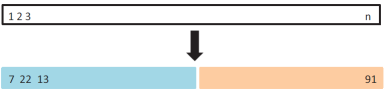
\includegraphics[width=.6\textwidth]{pictures/cross_validation_validation_set.png}
	\end{center}

	\paragraph{Leave-one-out cross-validation (LOOCV)}
	(image)
	Again, LOOCV splits the observations into two parts, but they are now not of comparable size, since only ONE observation is used for the validation set. Now the model can be fitted to almost all data (n-1) and then the prediction is made for the one single sample that was left out.Hence the MSE of this single sample is an approximately unbiased estimate of the test MSE, but it has a high variance. This variance can be reduced by repeating the procedure by systematically leaving out one sample after the other and then averaging the resulting single sample MSEs.
	\begin{equation}
		CV_{(n)}=\frac{1}{n}\sum_{i=1}^{n}MSE_{i}
	\end{equation}
	The main advantages are that (n-1) data points are used to fit the model instead of n/2 and there is no randomness in the procedure.
	Whatever, LOOCV is computationally quite expensive, since the model has to be fitted n times.\\
	There is one great exception for least squares linear (or polynomial) regression.
	\begin{equation}
	\begin{split}
		CV_{(n)}&=\frac{1}{n}\sum_{i=1}^{n}(\frac{y_{i}-\hat{y}_{i}}{1-h_{i}})^2\\
		h_{i}&=\frac{1}{n}+\frac{(x_{i}-\overline{x})^2}{\sum_{i'=1}^{n}(x_{i'}-\overline{x})^2}
	\end{split}
	\end{equation}
	What makes this formula powerful is the fact, that the model needs to fitted only once to all the data.
	\begin{center}
		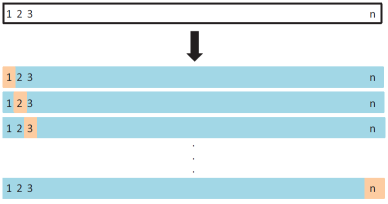
\includegraphics[width=.6\textwidth]{pictures/cross_validation_LOOCV.png}
	\end{center}

	\paragraph{k-fold cross-validation}
	(image)
	k-fold cross validation improves the LOOCV, so that it isn't so computationally expensive. The basic idea is to split the observations randomly in k equally sized sets. Clearly LOOCV is a special case of k-fold cross-validation, where k=n.
	\begin{equation}
		CV_{(k)}=\frac{1}{k}\sum_{i=1}^{k}MSE_{i}
	\end{equation}
	\begin{center}
		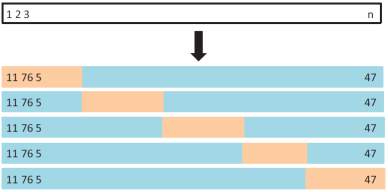
\includegraphics[width=.6\textwidth]{pictures/cross_validation_k_fold.png}
	\end{center}

	\paragraph{Bias-variance trade-off for k-fold cross-validation}
	\begin{itemize}
		\item The validation set method has the largest bias and the largest variance for estimating the true test MSE.
		\item The k-fold cross-validation has a medium bias and a low variance.
		\item The LOOCV has a low bias and a medium variance.

	\end{itemize}

	\subsection{The bootstrap}
	\begin{center}
		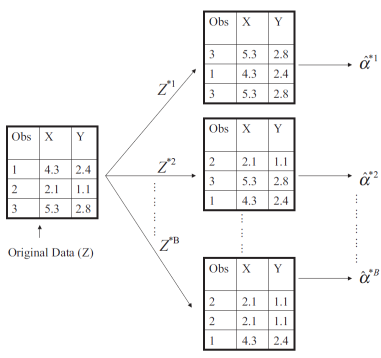
\includegraphics[width=0.8\textwidth]{pictures/bootstrap.png}
	\end{center}
	Method for quantifying the uncertainty associated with a given estimator or statistical learning method. The bootstrap method allows us to emulate the process of obtaining new samples sets. This is achieved by repeatedly sampling observations from the original data set.
	The sampling is performed with replacement, meaning the observation stays in the data set and can be selected (at random) again.
\end{document}
